\section{Теория}
	Случайный процесс протекающий в некоторой системе S называется марковским если он обладает следующим свойством. Для каждого момента времени $t_0$ вероятность любого состояния системы в будущем зависит \textbf{только} от её состояния в настоящем и не зависит от того как и когда она пришла в это состояние.
	
	Для марковского процесса обычно составляются уравнения Колмогорова: 
	\begin{equation*}
		F = (P'(t), P(t), \lambda) = 0
	\end{equation*}
	Где $\lambda$ - набор параметров 
	Интегрирование системы уравнений даёт исходные вероятности как функции времени. Также для решения необходимо условие нормировки $\sum_{i}^{n}{p_i} = 1$ 

\section{Работа программы}
	Условием стабилизации вероятности состояния $i$ принимается величина $P_i(t_{stab})$, где $t_{stab}$ - наименьшее время, при котором ${P'}_i(t_{stab}) < 10^{-7}$. 
	
	Примеры работы программы при различном количестве состояний и заполнении матрицы интенсивности приведены на рисунках \ref{pic:1}, \ref{pic:2} и \ref{pic:3}.
	
	\newpage
	\begin{figure}[h]
		\begin{center}
			{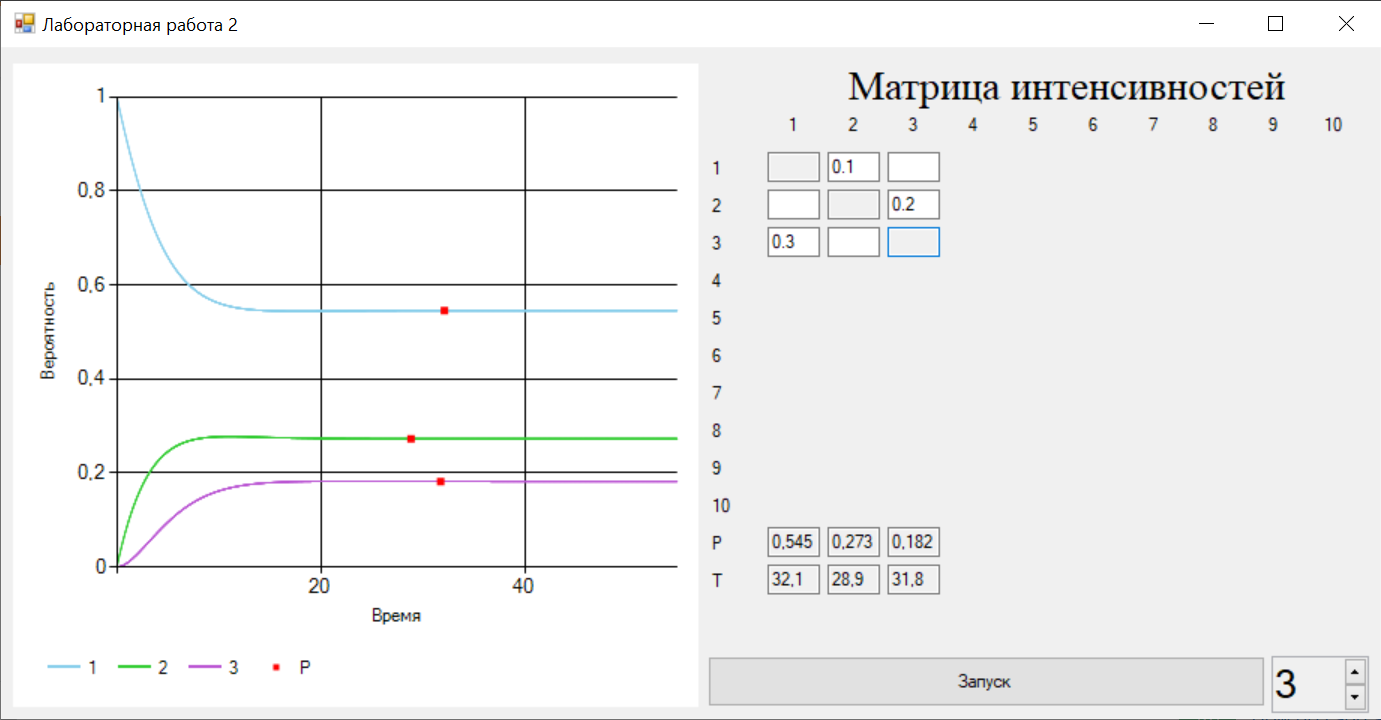
\includegraphics[scale=0.7]{1.png}
			\caption{Графики вероятностей состояний}
			\label{pic:1}}
		\end{center}
	\end{figure}
	
	Проверка результатов:
	\begin{equation}
		\left\{\begin{array}{l}
			-0.1 \cdot 0.545 + 0.3\cdot0.182 = 1.0\cdot10^{-4} \\
			-0.2 \cdot 0.273 + 0.1\cdot0.545 = -1.0\cdot10^{-4} \\
			-0.3 \cdot 0.182 + 0.2\cdot0.273 = 0.0
		\end{array}\right.
	\end{equation}
	
	Вычислим стабилизировавшиеся значения $P_1, P_2, P_3$:
	\begin{equation*}
		\left\{\begin{array}{l}
			-0.1 \cdot P_1 + 0.3 \cdot P_3 = 0 \\
			-0.2 \cdot P_2 + 0.1 \cdot P_1 = 0 \\
			-0.3 \cdot P_3 + 0.2 \cdot P_2 = 0 \\
			P_1 + P_2 + P_3 = 1
		\end{array}\right.
	\end{equation*}

	\begin{equation*}
		\left\{\begin{array}{l}
			P_1 = 3 \cdot P_3 \\
			P_2 = 1.5 \cdot P_3 \\
			5.5 \cdot P_3  = 1
		\end{array}\right.
	\end{equation*}

	\begin{equation*}
		\left\{\begin{array}{l}
			P_1 = \frac{6}{11} \\
			P_2 = \frac{3}{11} \\
			P_3  = \frac{2}{11}
		\end{array}\right.
	\end{equation*}
	
	Вычисленные аналитически значения совпадают со значениями, полученными программно
	
	\newpage
	\begin{figure}[h]
		\begin{center}
			{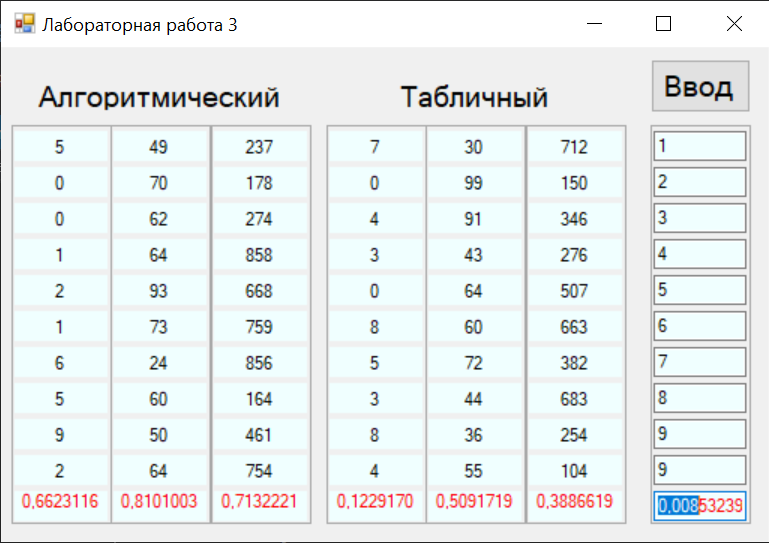
\includegraphics[scale=0.7]{2.png}
			\caption{Графики вероятностей состояний}
			\label{pic:2}}
		\end{center}
	\end{figure}

	Проверка результатов:
	\begin{equation}
		\left\{\begin{array}{l}
			-0.1\cdot0.375 + 0.1 \cdot 0.375 = 0.0 \\
			-(0.1+0.1)\cdot0.375 + (0.1\cdot0.375 + 0.2\cdot0.187) = -1.0\cdot10^{-4} \\
			-(0.2+0.1)\cdot0.187 + (0.1\cdot0.375 + 0.3\cdot0.062) = 0.0 \\
			-0.3\cdot0.062 + 0.1\cdot0.187 = 1.0\cdot10^{-4}
		\end{array}\right.
	\end{equation}
	
	\newpage
	\begin{figure}[h]
		\begin{center}
			{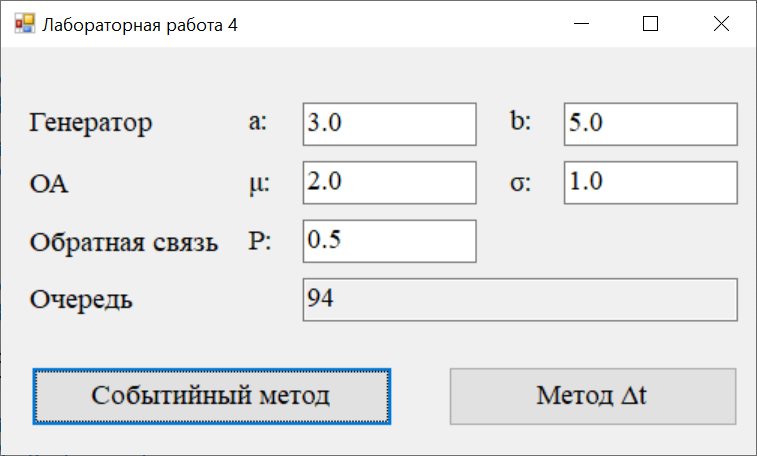
\includegraphics[scale=0.7]{3.png}
			\caption{Графики вероятностей состояний}
			\label{pic:3}}
		\end{center}
	\end{figure}

	Проверка результатов: 4-е состояние не имеет исходящее интенсивности, поэтому при $t \rightarrow \inf$ вероятность 4-го состояния должна равняться 0.
